\documentclass[12pt, a4paper]{article}

\usepackage{amsmath}
\usepackage{array}
\usepackage{amsmath}
\usepackage[portuguese]{babel}
\usepackage{chngpage}
\usepackage{float}
\usepackage[a4paper, margin=2cm]{geometry}
\usepackage{graphicx}
\usepackage{hyperref}
\usepackage{listings}
\usepackage{setspace}
\usepackage{xcolor}

\lstdefinestyle{codestyle}{
    commentstyle=\color{teal},
    keywordstyle=\color{blue},
    numberstyle=\ttfamily\color{gray},
    stringstyle=\color{red},
    basicstyle=\ttfamily\footnotesize,
    breakatwhitespace=false,
    breaklines=false,
    keepspaces=true,
    numbers=none,
    showspaces=false,
    showstringspaces=false,
    showtabs=false,
    tabsize=4
}
\lstset{style=codestyle}

\title{\Huge \textbf{Computação Gráfica \\ \Large Trabalho Prático -- Fase II}}
\date{30 de março 2025}
\author{Grupo 3}

\begin{document}

\begin{center}
    
\includegraphics[width=0.25\textwidth]{res/cover/EE-C.eps}
\end{center}

\chardef\_=`_
\onehalfspacing
\setlength{\parskip}{\baselineskip}
\setlength{\parindent}{0pt}
\def\arraystretch{1.5}

{\let\newpage\relax\maketitle}
\maketitle
\thispagestyle{empty}

\vspace*{\fill}

\begin{adjustwidth}{-2cm}{-2cm} % These values only need to be large enough to center the table
    \begin{center}
        \begin{tabular}{>{\centering}p{0.25\textwidth}
                        >{\centering}p{0.25\textwidth}
                        >{\centering}p{0.25\textwidth}
                        >{\centering\arraybackslash}p{0.25\textwidth}}
            
\includegraphics[width=3.5cm]{res/cover/A104437.png} &
            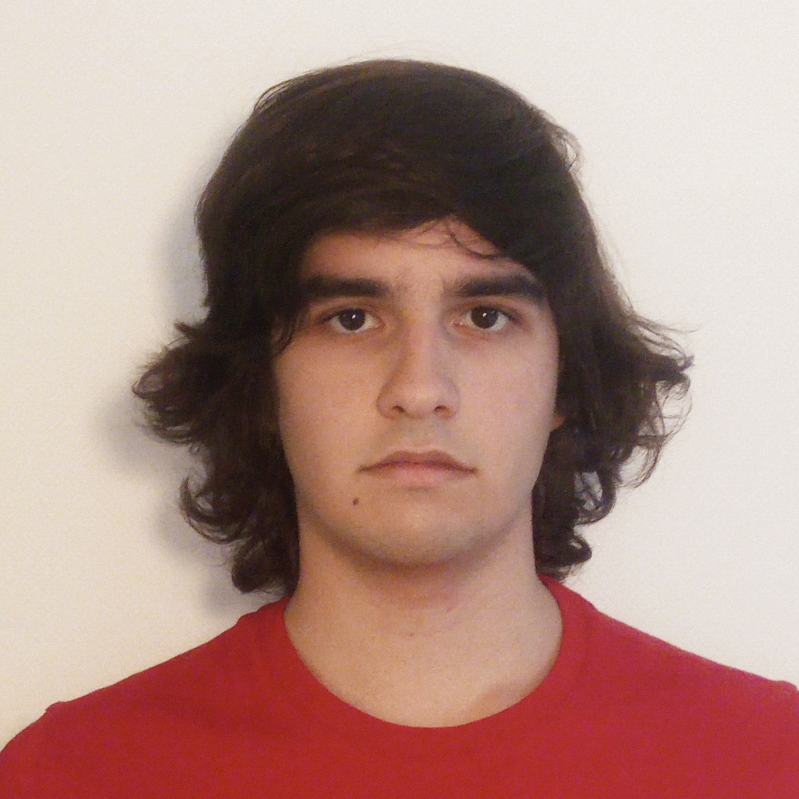
\includegraphics[width=3.5cm]{res/cover/A104348.png} &
            
\includegraphics[width=3.5cm]{res/cover/A90817.png} &
            
\includegraphics[width=3.5cm]{res/cover/A104179.png} \\

            Ana Oliveira & Humberto Gomes & Mariana Cristino & Sara Lopes \\
            A104437      & A104348        & A90817           & A104179
        \end{tabular}
    \end{center}
\end{adjustwidth}

\pagebreak

\begin{abstract}
    \textbf{\color{red} TODO - resumo}
\end{abstract}

\section{Transformações}

\textbf{\color{red} TODO - transformações}

\section{Modelo estático do sistema solar}

\textbf{\color{red} TODO - sistema solar}

\section{Extras}

Nesta fase, fizemos vários extras:
\begin{itemize}
    \item Geração de Möbius Strip;
    \item \color{red} TODO
    \item \color{red} TODO
    \item \color{red} TODO
\end{itemize}
\subsection{\emph{Möbius Strip}}

Para gerar um \emph{möbius strip} temos de ter um raio, uma largura, o número
de voltas, o número de slices, o número de stacks e o ficheiro onde iremos
colocar os vértices e as faces desta figura:
\begin{verbatim}
    ./generator mobiusStrip <radius> <width> <twist> <slices> <stacks> <file>
\end{verbatim}

Matematicamente, as coordenadas de um ponto do \emph{möbius strip} são definidas do seguinte modo:

$$x = (radius + \theta \times \frac{width}{2} \times \cos (\frac{twist \times \phi}{2})) \times
\cos (\phi)$$
$$y = radius \times \theta \times \frac{width}{2} \times \sin (\frac{twist \times \phi}{2})$$
$$z = (radius + \theta \times \frac{width}{2} \times \cos (\frac{twist \times \phi}{2})) \times
\sin (\phi)$$

$$\theta \in \left [ 0, 2 \pi \right [$$
$$\phi \in \left [ -1, 1 \right ]$$

\begin{figure}[H]
    \centering
    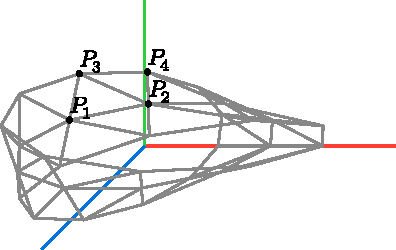
\includegraphics[width=0.35\textwidth]{res/phase2/figures/MobiusStrip.pdf}
    \caption{Faces do \emph{möbius strip} geradas numa iteração.}
\end{figure}

$$
T_1 = (P_1, P_2, P_3)
\hspace{1cm}
T_2 = (P_2, P_1, P_3)
\hspace{1cm}
T_3 = (P_3, P_2, P_4)
\hspace{1cm}
T_4 = (P_2, P_3, P_4)
$$


\textbf{\color{red} TODO - extras continuação}

\section{Resultados obtidos}

\textbf{\color{red} TODO - resultados}

\section{Conclusão e Trabalho Futuro}

\textbf{\color{red} TODO - conclusão}

\begingroup
\section{Bibliografia}
\renewcommand{\section}[2]{}

\begin{thebibliography}{9}
    \bibitem{exemplo}
        \href{https://youtu.be/dQw4w9WgXcQ}{Um item de exemplo na bibliografia}
\end{thebibliography}
\endgroup

\end{document}
